\section{Premica}

\begin{frame}
    \sectionpage
\end{frame}

\begin{frame}
    \tableofcontents[currentsection, hideothersubsections]
\end{frame}
        


    \subsection{Enačba premice}

        \begin{frame}
            \frametitle{Enačba premice}

            \begin{alertblock}{Eksplicitna oblika enačbe premice}
                $$ \mathbf{y=kx+n};~ k,n\in\mathbb{R},$$
                kjer je $k$ je \textbf{smerni koeficient}, ki ga izračunamo kot $$k=\dfrac{\Delta x}{\Delta y}=\dfrac{y_2-y_1}{x_2-x_1},$$                
                $n$ pa je \textbf{začetna vrednost}.
            \end{alertblock}

            \begin{block}{}
                Z eksplicitno obliko enačbe premice lahko zapišemo vse premice, razen tistih, ki so vzporedne ordinatni osi.
            \end{block}
        \end{frame}

        \begin{frame}
            \begin{block}{}
                Dana je premica, ki poteka skozi točki $(x_1,y_1)$ in $(x_2,y_2)$. \\
                Smerni koeficient izračunamo po formuli $$k=\dfrac{y_2-y_1}{x_2-x_1}.$$
                Iz $y_1=kx_1+n$ izrazimo $$n=y_1-kx_1$$
                in vstavimo v prvotno enačbo $$y=kx+y_1-kx_1$$
                ter preuredimo do oblike $$\mathbf{y-y_1=k(x-x_1)}.$$
            \end{block}
        \end{frame}


        \begin{frame}
            \begin{alertblock}{Odsekovna/segmentna oblika enačbe premice}
                Denimo, da premica seka koordinatni osi v točkah $M(m,0)$ in $N(0,n)$. \\
                Uporabimo eksplicitno obliko enačbe premice, v katero vstavimo znani točki
                $$y-0=\dfrac{n-0}{0-m}(x-m)$$ $$y=-\dfrac{n}{m}x+n,$$
                in  jo preoblikujemo do \textbf{odsekovne oblike enačbe premice}: 
                $$\mathbf{\dfrac{x}{m}+\dfrac{y}{n}=1}; ~m,n\in\mathbb{R}\setminus\{0\}.$$
            \end{alertblock}

            \begin{block}{}
                Vrednosti $m$ in $n$ določata \textbf{odseka}/\textbf{segmenta} na koordinatnih oseh.
            \end{block}

        \end{frame}


        \begin{frame}
            \begin{block}{}
                Z odsekovno obliko enačbe premice lahko zapišemo vse premice, razen tistih, 
                ki potekajo skozi koordinatno izhodišče $(0,0)$ ali pa so vzporedne eni od koordinatnih osi.
            \end{block}

            \begin{alertblock}{Implicitna oblika enačbe premice}
                Vsako premico lahko zapišemo z \textbf{implicitno obliko enačbe premice}:
                $$\mathbf{ax+by+c=0}; ~(a,b,c\in\mathbb{R}) \land (a~in~b~ne~hkrati~0).$$
            \end{alertblock}            
        \end{frame}


        %%%%% naloge

        \begin{frame}
            \only<2->{\begin{exampleblock}{Naloga}
                Narišite premico z dano eksplicitno obliko enačbe.
                    \begin{itemize}
                        \item $y=-2x+1$
                        \item $y=\dfrac{1}{2}x+2$
                        \item $y=2x+\dfrac{3}{4}$
                    \end{itemize}
            \end{exampleblock}}

            \only<3->{\begin{exampleblock}{Naloga}
                Narišite premico z dano odsekovno obliko enačbe.
                \vskip-1em
                \begin{columns}
                    \column{0.5\textwidth}
                    \begin{itemize}
                        \item $\dfrac{x}{3}+\dfrac{y}{5}=1$
                        \item $\dfrac{x}{2}+\dfrac{2y}{5}=1$
                    \end{itemize}

                    \column{0.47\textwidth}
                    \begin{itemize}
                        \item $\dfrac{x}{2}-\dfrac{y}{4}=1$
                        \item $\dfrac{x}{2}-\dfrac{y}{3}=-1$
                    \end{itemize}
                \end{columns}
            \end{exampleblock}}
        \end{frame}


                \begin{frame}
            \only<2->{\begin{exampleblock}{Naloga}
                Z grafa razberite ničlo in začetno vrednost ter zapišite odsekovno obliko enačbe premice.

                \begin{columns}
                    \column{0.32\textwidth}
                    \vskip-1.5em
                    \begin{figure}[H]
                        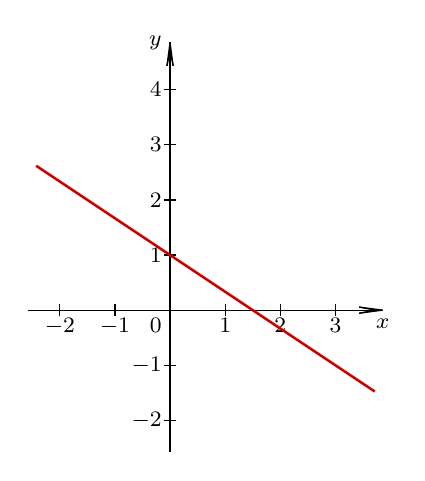
\begin{tikzpicture}
                            % \clip (0,0) rectangle (14.000000,10.000000);
                            {\footnotesize
                            
                            % Drawing 2D Cartesian system
                            \draw (3.000000,3.000000) node [anchor=north east] { $0$ };%
                            \draw [line width=0.016cm] (3.000000,2.925000) -- (3.000000,3.075000);%
                            \draw (3.700000,3.000000) node [anchor=north] { $1$ };%
                            \draw [line width=0.016cm] (3.700000,2.925000) -- (3.700000,3.075000);%
                            \draw (4.400000,3.000000) node [anchor=north] { $2$ };%
                            \draw [line width=0.016cm] (4.400000,2.925000) -- (4.400000,3.075000);%
                            \draw (5.100000,3.000000) node [anchor=north] { $3$ };%
                            \draw [line width=0.016cm] (5.100000,2.925000) -- (5.100000,3.075000);%
                            \draw (2.300000,3.000000) node [anchor=north] { $-1$ };%
                            \draw [line width=0.016cm] (2.300000,2.925000) -- (2.300000,3.075000);%
                            \draw (1.600000,3.000000) node [anchor=north] { $-2$ };%
                            \draw [line width=0.016cm] (1.600000,2.925000) -- (1.600000,3.075000);%
                            \draw (3.000000,3.700000) node [anchor=east] { $1$ };%
                            \draw [line width=0.016cm] (2.925000,3.700000) -- (3.075000,3.700000);%
                            \draw (3.000000,4.400000) node [anchor=east] { $2$ };%
                            \draw [line width=0.016cm] (2.925000,4.400000) -- (3.075000,4.400000);%
                            \draw (3.000000,5.100000) node [anchor=east] { $3$ };%
                            \draw [line width=0.016cm] (2.925000,5.100000) -- (3.075000,5.100000);%
                            \draw (3.000000,5.800000) node [anchor=east] { $4$ };%
                            \draw [line width=0.016cm] (2.925000,5.800000) -- (3.075000,5.800000);%
                            \draw (3.000000,2.300000) node [anchor=east] { $-1$ };%
                            \draw [line width=0.016cm] (2.925000,2.300000) -- (3.075000,2.300000);%
                            \draw (3.000000,1.600000) node [anchor=east] { $-2$ };%
                            \draw [line width=0.016cm] (2.925000,1.600000) -- (3.075000,1.600000);%
                            \draw (5.700000,3.000000) node [anchor=north] { $x$ };%
                            \draw (3.000000,6.400000) node [anchor=east] { $y$ };%
                            \draw [line width=0.016cm] (1.200000,3.000000) -- (5.700000,3.000000);%
                            \draw [line width=0.016cm] (5.402567,3.039158) -- (5.700000,3.000000);%
                            \draw [line width=0.016cm] (5.402567,3.039158) -- (5.600000,3.000000);%
                            \draw [line width=0.016cm] (5.402567,2.960842) -- (5.700000,3.000000);%
                            \draw [line width=0.016cm] (5.402567,2.960842) -- (5.600000,3.000000);%
                            \draw [line width=0.016cm] (3.000000,1.200000) -- (3.000000,6.400000);%
                            \draw [line width=0.016cm] (2.960842,6.102567) -- (3.000000,6.400000);%
                            \draw [line width=0.016cm] (2.960842,6.102567) -- (3.000000,6.300000);%
                            \draw [line width=0.016cm] (3.039158,6.102567) -- (3.000000,6.400000);%
                            \draw [line width=0.016cm] (3.039158,6.102567) -- (3.000000,6.300000);%
                            
                            % Changing color 204 0 0
                            \definecolor{r204g0b0}{rgb}{0.800000,0.000000,0.000000}%
                            \color{r204g0b0}% 
                            
                            % Drawing line l
                            \draw [line width=0.032cm] (1.300000,4.833220) -- (5.600000,1.966840);%
                            \color{black}
                            }
                            \end{tikzpicture}
                                                        
                    \end{figure}

                    \column{0.32\textwidth}
                    \vskip-1.5em
                    \begin{figure}[H]
                        \begin{tikzpicture}
                            % \clip (0,0) rectangle (14.000000,10.000000);
                            {\footnotesize
                            
                            % Drawing 2D Cartesian system
                            \draw (3.000000,3.000000) node [anchor=north east] { $0$ };%
                            \draw [line width=0.016cm] (3.000000,2.925000) -- (3.000000,3.075000);%
                            \draw (3.700000,3.000000) node [anchor=north] { $1$ };%
                            \draw [line width=0.016cm] (3.700000,2.925000) -- (3.700000,3.075000);%
                            \draw (4.400000,3.000000) node [anchor=north] { $2$ };%
                            \draw [line width=0.016cm] (4.400000,2.925000) -- (4.400000,3.075000);%
                            \draw (5.100000,3.000000) node [anchor=north] { $3$ };%
                            \draw [line width=0.016cm] (5.100000,2.925000) -- (5.100000,3.075000);%
                            \draw (2.300000,3.000000) node [anchor=north] { $-1$ };%
                            \draw [line width=0.016cm] (2.300000,2.925000) -- (2.300000,3.075000);%
                            \draw (1.600000,3.000000) node [anchor=north] { $-2$ };%
                            \draw [line width=0.016cm] (1.600000,2.925000) -- (1.600000,3.075000);%
                            \draw (3.000000,3.700000) node [anchor=east] { $1$ };%
                            \draw [line width=0.016cm] (2.925000,3.700000) -- (3.075000,3.700000);%
                            \draw (3.000000,4.400000) node [anchor=east] { $2$ };%
                            \draw [line width=0.016cm] (2.925000,4.400000) -- (3.075000,4.400000);%
                            \draw (3.000000,5.100000) node [anchor=east] { $3$ };%
                            \draw [line width=0.016cm] (2.925000,5.100000) -- (3.075000,5.100000);%
                            \draw (3.000000,5.800000) node [anchor=east] { $4$ };%
                            \draw [line width=0.016cm] (2.925000,5.800000) -- (3.075000,5.800000);%
                            \draw (3.000000,2.300000) node [anchor=east] { $-1$ };%
                            \draw [line width=0.016cm] (2.925000,2.300000) -- (3.075000,2.300000);%
                            \draw (3.000000,1.600000) node [anchor=east] { $-2$ };%
                            \draw [line width=0.016cm] (2.925000,1.600000) -- (3.075000,1.600000);%
                            \draw (5.700000,3.000000) node [anchor=north] { $x$ };%
                            \draw (3.000000,6.400000) node [anchor=east] { $y$ };%
                            \draw [line width=0.016cm] (1.200000,3.000000) -- (5.700000,3.000000);%
                            \draw [line width=0.016cm] (5.402567,3.039158) -- (5.700000,3.000000);%
                            \draw [line width=0.016cm] (5.402567,3.039158) -- (5.600000,3.000000);%
                            \draw [line width=0.016cm] (5.402567,2.960842) -- (5.700000,3.000000);%
                            \draw [line width=0.016cm] (5.402567,2.960842) -- (5.600000,3.000000);%
                            \draw [line width=0.016cm] (3.000000,1.200000) -- (3.000000,6.400000);%
                            \draw [line width=0.016cm] (2.960842,6.102567) -- (3.000000,6.400000);%
                            \draw [line width=0.016cm] (2.960842,6.102567) -- (3.000000,6.300000);%
                            \draw [line width=0.016cm] (3.039158,6.102567) -- (3.000000,6.400000);%
                            \draw [line width=0.016cm] (3.039158,6.102567) -- (3.000000,6.300000);%
                            
                            % Changing color 204 0 0
                            \definecolor{r204g0b0}{rgb}{0.800000,0.000000,0.000000}%
                            \color{r204g0b0}% 
                            
                            % Drawing line l
                            \draw [line width=0.032cm] (2.700000,1.300000) -- (5.600000,4.200000);%
                            \color{black}
                            }
                            \end{tikzpicture}
                            
                    \end{figure}

                    \column{0.32\textwidth}
                    \vskip-1.5em
                    \begin{figure}[H]
                        \begin{tikzpicture}
                            % \clip (0,0) rectangle (14.000000,10.000000);
                            {\footnotesize
                            
                            % Drawing 2D Cartesian system
                            \draw (3.000000,3.000000) node [anchor=north east] { $0$ };%
                            \draw [line width=0.016cm] (3.000000,2.925000) -- (3.000000,3.075000);%
                            \draw (3.700000,3.000000) node [anchor=north] { $1$ };%
                            \draw [line width=0.016cm] (3.700000,2.925000) -- (3.700000,3.075000);%
                            \draw (4.400000,3.000000) node [anchor=north] { $2$ };%
                            \draw [line width=0.016cm] (4.400000,2.925000) -- (4.400000,3.075000);%
                            \draw (5.100000,3.000000) node [anchor=north] { $3$ };%
                            \draw [line width=0.016cm] (5.100000,2.925000) -- (5.100000,3.075000);%
                            \draw (2.300000,3.000000) node [anchor=north] { $-1$ };%
                            \draw [line width=0.016cm] (2.300000,2.925000) -- (2.300000,3.075000);%
                            \draw (1.600000,3.000000) node [anchor=north] { $-2$ };%
                            \draw [line width=0.016cm] (1.600000,2.925000) -- (1.600000,3.075000);%
                            \draw (3.000000,3.700000) node [anchor=east] { $1$ };%
                            \draw [line width=0.016cm] (2.925000,3.700000) -- (3.075000,3.700000);%
                            \draw (3.000000,4.400000) node [anchor=east] { $2$ };%
                            \draw [line width=0.016cm] (2.925000,4.400000) -- (3.075000,4.400000);%
                            \draw (3.000000,5.100000) node [anchor=east] { $3$ };%
                            \draw [line width=0.016cm] (2.925000,5.100000) -- (3.075000,5.100000);%
                            \draw (3.000000,5.800000) node [anchor=east] { $4$ };%
                            \draw [line width=0.016cm] (2.925000,5.800000) -- (3.075000,5.800000);%
                            \draw (3.000000,2.300000) node [anchor=east] { $-1$ };%
                            \draw [line width=0.016cm] (2.925000,2.300000) -- (3.075000,2.300000);%
                            \draw (3.000000,1.600000) node [anchor=east] { $-2$ };%
                            \draw [line width=0.016cm] (2.925000,1.600000) -- (3.075000,1.600000);%
                            \draw (5.700000,3.000000) node [anchor=north] { $x$ };%
                            \draw (3.000000,6.400000) node [anchor=east] { $y$ };%
                            \draw [line width=0.016cm] (1.200000,3.000000) -- (5.700000,3.000000);%
                            \draw [line width=0.016cm] (5.402567,3.039158) -- (5.700000,3.000000);%
                            \draw [line width=0.016cm] (5.402567,3.039158) -- (5.600000,3.000000);%
                            \draw [line width=0.016cm] (5.402567,2.960842) -- (5.700000,3.000000);%
                            \draw [line width=0.016cm] (5.402567,2.960842) -- (5.600000,3.000000);%
                            \draw [line width=0.016cm] (3.000000,1.200000) -- (3.000000,6.400000);%
                            \draw [line width=0.016cm] (2.960842,6.102567) -- (3.000000,6.400000);%
                            \draw [line width=0.016cm] (2.960842,6.102567) -- (3.000000,6.300000);%
                            \draw [line width=0.016cm] (3.039158,6.102567) -- (3.000000,6.400000);%
                            \draw [line width=0.016cm] (3.039158,6.102567) -- (3.000000,6.300000);%
                            
                            % Changing color 204 0 0
                            \definecolor{r204g0b0}{rgb}{0.800000,0.000000,0.000000}%
                            \color{r204g0b0}% 
                            
                            % Drawing line l
                            \draw [line width=0.032cm] (4.900000,6.300000) -- (1.300000,2.700000);%
                            \color{black}
                            }
                            \end{tikzpicture}
                            
                    \end{figure}

                \end{columns}

            \end{exampleblock}}

        \end{frame}


        \begin{frame}
            \only<2->{\begin{exampleblock}{Naloga}
                Dano enačbo premice zapišite v eksplicitni in odsekovni obliki ter premico narišite.
                \vskip-1em
                \begin{columns}
                    \column{0.5\textwidth}
                    \begin{itemize}
                        \item $x+4y-8=0$
                        \item $3x-2y+6=0$
                        \item $2x+5y+5=0$
                    \end{itemize}

                    \column{0.47\textwidth}
                    \begin{itemize}
                        \item $\dfrac{1}{2}x+3y-6=0$
                        \item $x+1=0$
                        \item $y-2=0$ \\~
                    \end{itemize}
                \end{columns}

            \end{exampleblock}}

            \only<3->{\begin{exampleblock}{Naloga}
                Izračunajte ploščino trikotnika, ki jo premica oklepa s koordinatnima osema.
                \vskip-1em
                \begin{columns}
                    \column{0.5\textwidth}
                    \begin{itemize}
                        \item $y=-2x+4$
                        \item $\dfrac{x}{2}+\dfrac{x}{-3}=1$
                    \end{itemize}

                    \column{0.47\textwidth}
                    \begin{itemize}
                        \item $2x+4y-3=0$
                        \item $x-y+1=0$ \\~
                    \end{itemize}
                \end{columns}
            \end{exampleblock}}

        \end{frame}


        \begin{frame}
            \only<2->{\begin{exampleblock}{Naloga}
                Zapišite enačbo premice, ki gre skozi dani točki.
                    \begin{itemize}
                        \item $A(2,3)$ in $B(4,5)$ 
                        \item $C(1,-2)$ in $D(-3,-4)$ 
                        \item $E(7,2)$ in $F(-7,-5)$ \\~
                    \end{itemize}
            \end{exampleblock}}

            \only<3->{\begin{exampleblock}{Naloga}
                Določite neznano koordinato tako, da bodo dane točke kolinearne.
                    \begin{itemize}
                        \item $A(3,y)$, $B(-4,1)$ in $C(2,2)$ 
                        \item $D(-1,7)$, $E(x,5)$ in $F(3,-4)$ \\~
                    \end{itemize}
            \end{exampleblock}}

        \end{frame}


        \begin{frame}
            \only<2->{\begin{exampleblock}{Naloga}
                Ugotovite, ali sta dani premici vzporedni.
                    \begin{itemize}
                        \item $y=\dfrac{3}{4}x-1$ in $y=-\dfrac{3}{4}x+1$ \\~
                        \item $x-2y+1=0$ in $2x+y+1=0$ \\~
                        \item $\dfrac{x}{3}-\dfrac{y}{6}=1$ in $\dfrac{x}{2}+\dfrac{y}{4}=1$ \\~
                        \item $\dfrac{x}{4}+\dfrac{y}{2}=1$ in $4x+2y+1=0$ \\~

                    \end{itemize}
            \end{exampleblock}}


        \end{frame}


        \begin{frame}
            
            \only<2->{\begin{exampleblock}{Naloga}
                Dani sta premici z enačbama $y=4x+9$ in $ax-3y+3=0$. Določite parameter $a$ tako, da bosta premici vzporedni.
            \end{exampleblock}}

            \only<3->{\begin{exampleblock}{Naloga}
                Dani sta premici z enačbama $\dfrac{x}{2}-\dfrac{y}{7}=1$ in $-6x+by+1=0$. Določite parameter $b$ tako, da bosta premici vzporedni.
            \end{exampleblock}}

            \only<4->{\begin{exampleblock}{Naloga}
                Dani sta premici z enačbama $3x-2y+4=0$ in $(c-2)x+4y+3=0$. Določite parameter $c$ tako, da bosta premici vzporedni.
            \end{exampleblock}}

        \end{frame}


        \begin{frame}
            \only<2->{\begin{exampleblock}{Naloga}
                Zapišite enačbo premice, ki je vzporedna dani premici in poteka skozi dano točko.
                    \begin{itemize}
                        \item $y=2x-1$, $T(1,-3)$ 
                        \item $2x-4y+3=0$, $U(-4,5)$ 
                        \item $\dfrac{x}{4}+\dfrac{y}{8}=1$, $V(8,-8)$ \\~

                    \end{itemize}
            \end{exampleblock}}


            \only<3->{\begin{exampleblock}{Naloga}
                Iz snopa premic z enačbo $y=-3x+n$ določite enačbo tiste premice, ki poteka skozi točko $(1,4)$.
            \end{exampleblock}}

            \only<4->{\begin{exampleblock}{Naloga}
                Iz šopa premic z enačbo $y=kx+2$ določite enačbo tiste premice, ki gre skozi točko $(3,-4)$.
            \end{exampleblock}}

        \end{frame}


        \begin{frame}
            \only<2->{\begin{exampleblock}{Naloga}
                Zapišite enačbo pravokotnice na dano premico, ki poteka skozi dano točko.
                    \begin{itemize}
                        \item $y=x+2$, $T(3,-4)$ \\~
                        \item $y=2x+3$, $U(4,5)$ \\~
                        \item $y=\dfrac{1}{3}x+5$, $V(-1,4)$ \\~
                        \item $y=-\dfrac{2}{3}x+\dfrac{4}{5}$, $Z(-6,3)$ \\~

                    \end{itemize}
            \end{exampleblock}}

        \end{frame}




    \subsection{Presečišče premic}

        \begin{frame}
            \frametitle{Presečišče premic}
        \end{frame}


        \begin{frame}
            \only<2->{\begin{exampleblock}{Naloga}
                Izračunajte presečišče premic, rezultat preverite s sliko.
                \begin{itemize}
                    \begin{columns}
                        \column{0.4\textwidth}
                        \item $\begin{aligned}
                            2x-3x-3&=0 \\ x&=3
                        \end{aligned}$ \\~\\~
                        \item $\begin{aligned}
                            y&=3x+3 \\ y&=\dfrac{x}{2}+3
                        \end{aligned}$ \\~

                        \column{0.4\textwidth}
                        \item $\begin{aligned}
                            x+3y-9&=0 \\ x-3y-3&=0
                        \end{aligned}$ \\~\\~
                        \item $\begin{aligned}
                            \dfrac{x}{3}-\dfrac{y}{6}&=1 \\ \dfrac{x}{2}+\dfrac{y}{5}&=1
                        \end{aligned}$ \\~
                    \end{columns}

                \end{itemize}
            \end{exampleblock}}
        \end{frame}


        \begin{frame}
            
            \only<2->{\begin{exampleblock}{Naloga}
                Zapišite enačbo premice, ki gre skozi presečišče premic $y=2x+1$ in $y=-\frac{1}{2}x+6$ ter seka ordinatno os pri $y=4$.
            \end{exampleblock}}

            \only<3->{\begin{exampleblock}{Naloga}
                Zapišite enačbo premice, ki gre skozi presečišče premic $y=3x+1$ in $y=-x+5$ ter ima smerni koeficient $k=2$.
            \end{exampleblock}}

            \only<4->{\begin{exampleblock}{Naloga}
                Zapišite implicitno enačbo premice, ki gre skozi presečišče premic $2x-y-13=0$ in $2x+3y-1=0$ ter seka abscisno os pri $x=\frac{7}{2}$.
            \end{exampleblock}}

        \end{frame}


        \begin{frame}
            
            \only<2->{\begin{exampleblock}{Naloga}
                Zapišite enačbo premice, ki gre skozi presečišče premic $3x+4y-11=0$ in $2x-7y+41=0$ ter je vzporedna ordinatni osi.
            \end{exampleblock}}

            \only<3->{\begin{exampleblock}{Naloga}
                Zapišite eksplicitno enačbo premice, ki gre skozi presečišče premic $5x-7y+3=0$ in $2x+y-14=0$ ter je vzporedna premici z enačbo $3x-2y+1=0$.
            \end{exampleblock}}

            \only<4->{\begin{exampleblock}{Naloga}
                Izračunajte smerni koeficient $k$ tako, da se premici z enačbama $y=2x+6$ in $y=kx+\frac{5}{2}$ sekata na simetrali sodih kvadrantov.
            \end{exampleblock}}

        \end{frame}


        \begin{frame}
            
            \only<2->{\begin{exampleblock}{Naloga}
                Stranice trikotnika ležijo na premicah z enačbami $x+y=0$, $3x-2y=0$ in $x-4y+10=0$. 
                Izračunajte oglišča trikotnika ter njegov obseg in ploščino.
                Premice in trikotnik narišite v pravokotnem koordinatnem sistemu.
            \end{exampleblock}}

            \only<3->{\begin{exampleblock}{Naloga}
                Dani sta dve oglišči $A$ in $B$ trikotnika $\triangle ABC$, orientacija in ploščina. Izračunajte kooridnati tretjega oglišča $C$, če leži na dani premici.
                \begin{itemize}
                    \item $A(-6,1)$, $B(2,-1)$; \\ pozitivna orientacija, $S=25$; \\ $C$ leži na $y=-2x+4$
                    \item $A(-4,0)$, $B(4,2)$; \\ pozitivna orientacija, $S=7$; \\ $C$ leži na $y=5-2x$
                \end{itemize}
            \end{exampleblock}}


        \end{frame}